%%==================================================================%%
%% Author : Abascal Fern�ndez, Patricia                             %%
%% Author : S�nchez Barreiro, Pablo                                 %%
%% Version: 1.0, 24/06/2013                                         %%
%%                                                                  %%
%% Memoria del Proyecto Fin de Carrera                              %%
%% Application Engineering/Modelo de Entrada                        %%
%%==================================================================%%

La estrategia para crear un modelo arquitect�nico concreto consiste, tal como se describi� en la Secci�n~\ref{sec:back:uml}, en crear un paquete vac�o, el cual representa el producto a construir, y a�adir relaciones \emph{merge} a aquellas caracter�sticas que se desean incluir en el producto final. De esta forma, el contenido de los paquetes correspondiente a caracter�sticas que se deben incluir en el producto final, se combinan o componen en el paquete que representa el producto final.

Para distinguir el paquete que representa el producto final de los paquetes que representan caracter�sticas, se ha creado un perfil de UML 2.0. Un perfil UML 2.0 es un mecanismo gen�rico de extensi�n que permite personalizar los modelos UML para un prop�sito particular, mediante la especificaci�n de estereotipos y valores etiquetados que modifican la sem�ntica original de los elementos del modelo UML 2.0.

\begin{figure}[!tb]
  \center
  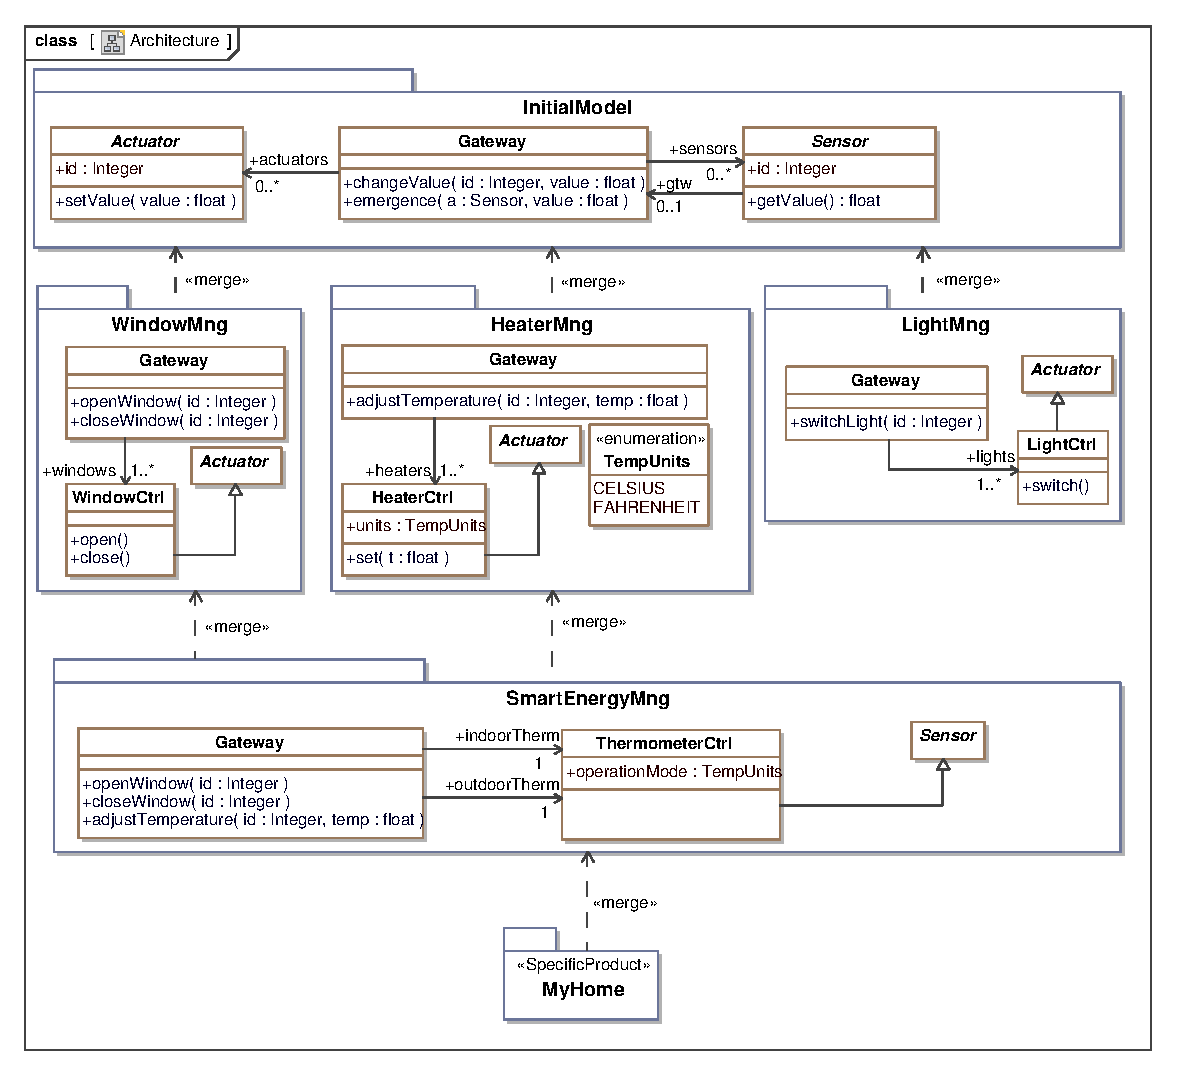
\includegraphics[width=0.75\linewidth]{applicationEngineering/images/Configuration(1).eps} \\
  \caption{Configuraci�n de un hogar inteligente completo}
  \label{app:fig:conf1}
\end{figure}

En nuestro caso, el perfil contiene un solo estereotipo, denominado \imp{SpecificProduct}, el cual se puede aplicar exclusivamente a paquetes UML tal como se puede apreciar en la Figura~\ref{app:fig:conf1}. Adem�s, por cada modelo UML 2.0 representando un producto concreto, s�lo puede existir un paquete estereotipado de dicha forma. Esta �ltima restricci�n se expresa por medio de OCL.\\

La Figura~\ref{app:fig:conf1} muestra un ejemplo de creaci�n de un producto concreto dentro de la l�nea de productos software para hogares inteligentes. En este caso, se trata de un producto donde se ha incluido exclusivamente la caracter�stica de \imp{SmartEnergyMng}, lo que implica que deben seleccionarse adem�s las caracter�sticas \imp{WindowMng} y \imp{HeaterMng}, ya que \imp{SmartEnergyMng} necesita que ambas caracter�sticas est�n instaladas en un producto final para poder funcionar. Dicha dependencia queda especificada de forma expl�cita a trav�s de las relaciones \emph{merge} existentes entre \imp{SmartEnergyMng} y \imp{WindowMng} y \imp{HeaterMng}. Debido a dichas relaciones, es imposible crear un producto que incluya \imp{SmartEnergyMng} pero no \imp{WindowMng} o \imp{HeaterMng}.

La siguiente secci�n describe c�mo este modelo arquitect�nico puede transformarse autom�ticamente en el c�digo necesario para crear una implementaci�n concreta y completamente funcional de un producto software concreto.

